% Selected verbatim passages from the source of:
% Christian Gaetz and Yibo Gao, "Balance constants for Coxeter groups",
% Trans. Amer. Math. Soc. 376 (2023), 8973--9000.
% doi:10.1090/tran/9040; arXiv:2005.09719v2.
% Target: Question 3.10 (not the general Conjecture 1.2).
% The order convention, word convention and all four figures matter.
\documentclass{amsart}
\usepackage{amsthm}
\usepackage{amsmath}
\usepackage{amssymb}
\usepackage{comment}
\usepackage{enumitem}
\usepackage{amsfonts}
\usepackage{mathtools}
\usepackage{hyperref}
\usepackage{tikz}
\usepackage[utf8]{inputenc}

\DeclareMathOperator{\conv}{Conv}
\DeclareMathOperator{\wid}{width}
\DeclareMathOperator{\cay}{Cay}

\DeclareMathOperator{\di}{\delta^{\text{ideal}}}
\DeclareMathOperator{\bi}{\textit{b}^{\text{ideal}}}

\newcommand{\mc}{\mathcal}
\newcommand{\mf}{\mathfrak}
\newcommand{\bs}{\boldsymbol}

\newcommand{\GL}{\mathrm{GL}}
\newcommand{\height}{\mathrm{ht}}
\newcommand{\R}{\mathbb{R}}
\newcommand{\Vol}{\mathrm{Vol}}
\newcommand{\id}{\mathrm{id}}
\renewcommand{\O}{\mathcal{O}}

\newcommand\precdot{\mathrel{\ooalign{$\prec$\cr
  \hidewidth\raise0.001ex\hbox{$\cdot\mkern0.6mu$}\cr}}}

\newtheorem{theorem}{Theorem}[section]
\newtheorem{def-prop}[theorem]{Definition-Proposition}
\newtheorem{prop}[theorem]{Proposition}
\newtheorem{conj}[theorem]{Conjecture}
\newtheorem{lemma}[theorem]{Lemma}
\newtheorem{cor}[theorem]{Corollary}

\theoremstyle{definition}
\newtheorem{ex}[theorem]{Example}
\newtheorem{quest}[theorem]{Question}
\newtheorem{defin}[theorem]{Definition}

\theoremstyle{remark}
\newtheorem*{remark}{Remark}
\begin{document}
\section*{Balance and the ambient conjecture}
For any convex set $C$ in a Coxeter group $W$ and any reflection $t$ we define
\[
\delta_C(t)=\frac{|C_t|}{|C|},
\]
where $C_t=\{w \in C \: | \: \ell(wt)<\ell(w)\}$ is the set of elements in $C$ having $t$ as an inversion; when $C$ is clear we often simply write $\delta(t)$.  In light of the discussion in Section~\ref{sec:intro-convex-sets} this definition is exactly analogous to (\ref{eq:def-delta-for-posets}), recovering $\delta_P(x,y)$ when $W=S_n$, $C$ is the convex set associated to $P$, and $t$ is the transposition swapping $\lambda(x)$ and $\lambda(y)$.  It thus makes sense to define the \emph{balance constant}
\[
b(C)=\max_t \min(\delta_C(t), 1-\delta_C(t)).
\]
Remarkably, when $W$ is a finite Weyl group, Conjecture~\ref{conj:1-3-2-3} appears still to hold:

\begin{conj}\label{conj:1-3-2-3-weyl}
Let $W$ be any finite Weyl group and $C \subseteq W$ a convex set which is not a singleton. Then $b(C) \geq \frac{1}{3}$.
\end{conj}
\section*{Order conventions}
We follow the conventions of \cite{Bjorner-Brenti}. Let $(W,S)$ be a Coxeter system.  We write $\Gamma$ for the associated \emph{Coxeter diagram}, the graph with vertex set $S$ and an edge labelled $m_{ij}$ between vertices $s_i$ and $s_j$ whenever the quantity $m_{ij}$ giving the defining relation $(s_is_j)^{m_{ij}}=\id$ of $W$ is at least $3$.  We say $W$ is \emph{acyclic} if the graph $\Gamma$ contains no cycles, and \emph{irreducible} if $\Gamma$ is connected.

For $w \in W$, the \emph{length} $\ell(w)$ is the smallest number $\ell$ such that $w=s_1 \cdots s_{\ell}$ with the $s_i \in S$.  Such an expression of minimal length is called a \emph{reduced word} or \emph{reduced expression}.  The \emph{left (resp. right) weak order} is the partial order on $W$ with cover relations $u \lessdot_L su$ (resp. $u \lessdot_R us)$ whenever $\ell(su)=\ell(u)+1$ (resp. $\ell(us)=\ell(u)+1$) and $s \in S$.  We write $\cay_L(W)$ and $\cay_R(W)$ for the left and right Cayley graphs for $W$ with respect to the generating set $S$, viewing these as undirected graphs, and often identifying them with the Hasse diagrams of the weak orders.

The set $T$ of conjugates of elements of $S$ is called the set of \emph{reflections}.  For $w \in W$ the \emph{right (resp. left) inversion set} $T_R(w)$ is $\{t \in T \: | \: \ell(wt)<\ell(w)\}$ (resp. $\{t \in T \: | \: \ell(tw)<\ell(w)\}$).  It is well known that
\[
|T_R(w)|=|T_L(w)|=\ell(w),
\]
and that weak order is characterized by containment of inversions sets:
\begin{align*}
   u &\leq_L v \iff T_R(u) \subseteq T_R(v) \\
   u &\leq_R v \iff T_L(u) \subseteq T_L(v).
\end{align*}

A subset $C \subseteq W$ is \emph{left (resp. right) convex} if it is convex with respect to the metric on $W$ determined by the natural graph distance in $\cay_L(W)$ (resp. $\cay_R(W)$).  That is, $C$ is convex if all elements of $W$ which lie on some minimum-length path in $\cay_L$ between $u$ and $v$ lie in $C$ whenever $u$ and $v$ do.  The \emph{left (resp. right) convex hull} $\conv_L(w_1,\ldots, w_d)$ (resp. $\conv_R(w_1,\ldots, w_d)$) of a collection of elements $w_1, \ldots, w_d \in W$ is defined to be the intersection of all left (resp. right) convex subsets of $W$ which contain $\{w_1,\ldots,w_d\}$; the convex hull is itself clearly convex.

\begin{remark}
We make the convention that when ``left" and ``right" are not specified it is assumed that we are working with left weak order, left Cayley graphs and convex sets, and so on.
\end{remark}
\section*{Fully commutative elements and their heaps}
For $(W,S)$ any Coxeter system and $w \in W$, we write $\mc{R}_w$ for the set of reduced words of $w$.  A well known result of Tits \cite{Tits-words} implies that all elements of $\mc{R}_w$ are connected by relations of the form
\[
s_is_j \cdots = s_js_i \cdots
\]
with $m_{ij} \geq 2$ factors on each side.  Applying such a relation to a reduced word is called a \emph{commutation move} when $m_{ij}=2$ and a \emph{braid move} otherwise.  Allowing only commutation moves determines an equivalence relation $\sim$ on $\mathcal{R}_w$, and the elements of $\mathcal{R}_w / \sim$ are called \emph{commutation classes}.

\begin{defin}[Stembridge \cite{Stembridge}]
An element $w \in W$ is called \emph{fully commutative} if $\mc{R}_w$ consists of a single commutation class.  Equivalently, $w$ is fully commutative if no reduced word for $w$ admits a braid move.
\end{defin}

Let $(W,S)$ be any Coxeter system. Given an element $w \in W$ with a reduced word $w=s_{i_1} \cdots s_{i_{\ell}}=\bs{s} \in \mc{R}_w$ the associated \emph{heap poset} (or just \emph{heap}) $H_{\bs{s}}$ is the partial order $([\ell], \preceq)$ which is the transitive closure of the following relation:
\[
j \preceq k \text{ if $j \geq k$ and $m_{i_j i_k} \neq 2$},
\]
where the $m_*$'s are the edge labels of the Coxeter diagram of $W$.  We also give heaps the structure of $S$-labelled posets by associating with the vertex $j$ the simple reflection $s_{i_j}$.  As we may have $i_j=i_{j'}$, multiple vertices may receive the same $S$-label.  Heaps were introduced in a more general setting by Viennot \cite{Viennot} and applied to reduced words in Coxeter groups by Stembridge \cite{Stembridge}.

\begin{prop}[Stembridge \cite{Stembridge}]
\label{prop:heap-depend-on-commutation-class}
The heap poset $H_{\bs{s}}$, as an $S$-labelled poset, depends only on the commutation class of $\bs{s}$.
\end{prop}

By Proposition~\ref{prop:heap-depend-on-commutation-class}, if $w$ is fully commutative the heap $H_{\bs{s}}$ does not depend on the chosen reduced word $\bs{s} \in \mc{R}_w$.  Thus we may refer unambiguously to the heap of $w$, which we denote by $H_w$.

Suppose that $w$ is fully commutative and $u \in [\id,w]_L$; clearly $u$ is also fully commutative.  Choose any reduced word $\bs{s'}=s_{i_{\ell'+1}} \cdots s_{i_{\ell}}$ for $u$ and construct the heap $H_w$ with respect to an augmented reduced word
\[
\bs{s}=s_{i_1} \cdots s_{i_{\ell'}} s_{i_{\ell'+1}} \cdots s_{i_{\ell}}=w.
\]
Since $\bs{s'}$ is a suffix of $\bs{s}$, it is immediate from the definitions that $H_w$ contains the $S$-labelled poset $H_u$ as an order ideal.  Thus we have constructed a map
\begin{align*}
\Psi: [\id,w]_L &\to J(H_w) \\
u & \mapsto H_u
\end{align*}
where, for a finite poset $P$, we write $J(P)$ for the distributive lattice of order ideals of $P$. (See \cite[\S 3.4]{ec1} for basic properties of $J(P)$.)  Furthermore, it is clear that $\Psi$ is order preserving.

\begin{prop}[Stembridge \cite{Stembridge}]
\label{prop:weak-order-interval-from-heap}
Let $w \in W$ be fully commutative. Then
\[
\Psi: [\id,w]_L \to J(H_w)
\]
is an isomorphism of posets.
\end{prop}

We may identify the poset $[\id,w]_L$ with the set of inversion sets $T_R(u)$ for $u \in [\id,w]_L$ ordered by containment. The isomorphism $\Psi$ between distributive lattices induces a bijection
\begin{align}
\label{eq:Psi-and-psi}
\psi: T_R(w) &\to H_w  \\
s_{i_{\ell}}s_{i_{\ell-1}}\cdots s_{i_{a+1}} s_{i_a} s_{i_{a+1}} &\cdots s_{i_{\ell-1}} s_{i_{\ell}} \mapsto a \nonumber
\end{align}
such that for any $u \in [\id,w]_L$ we have
\[
\Psi(u)=\{\psi(t) \: | \: t \in T_R(u)\} \in J(H_w).
\]

This observation immediately implies the following proposition, which will be crucial to our proof of Conjecture~\ref{conj:1-3-2-3-weyl} for fully commutative elements in acyclic Coxeter groups in Section \ref{sec:fc-theorem}.

\begin{prop}
\label{prop:inversion-fraction-equals-ideal-fraction}
Let $W$ be any Coxeter group. Let $w\in W$ be fully commutative and $C=[\id,w]_L$; let $\psi: T_R(w) \to H_w$ be as in (\ref{eq:Psi-and-psi}).  Then for any $t \in T_R(w)$ and $x=\psi(t) \in H_w$ we have
\[
\delta_C(t)=\frac{|\{I \in J(H_w) \: | \: x \in I\}|}{|J(H_w)|}.
\]

\end{prop}

In light of Proposition~\ref{prop:inversion-fraction-equals-ideal-fraction} we will use the notation
\begin{align*}
    \di(x; Q) &= \frac{|\{I \in J(Q) \: | \: x \in I\}|}{|J(Q)|}, \\
    \bi(Q) &= \max_x \min(\di(x; Q), 1-\di(x; Q)),
\end{align*}
and sometimes write just $\di(x)$ when $Q$ is clear from context.
\section*{The four figures and the question}
\begin{figure}[ht!]
\centering
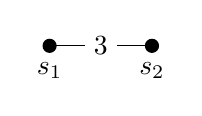
\begin{tikzpicture}
\node[draw,shape=circle,fill=black,scale=0.5](a)[label=below: {$s_1$}] at (-0.3,0) {};
\node[draw,shape=circle,fill=black,scale=0.5](b)[label=below: {$s_2$}] at (1,0) {};

\draw (b)--(a) node [midway, fill=white] {$3$};
\end{tikzpicture}
\hspace{0.5in}
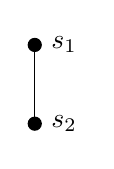
\begin{tikzpicture}
\node[draw,shape=circle,fill=black,scale=0.5](a)[label=right: {$s_2$}] at (0,0) {};
\node[draw,shape=circle,fill=black,scale=0.5](d)[label=right: {$s_1$}] at (0,1) {};

\draw (a)--(d);
\end{tikzpicture}
\caption{The Coxeter diagram (left) for the Weyl group of type $A_2$ (the symmetric group $S_3$). The fully commutative element $w=s_1s_2=231$ has heap poset $H_w$ shown on the right with $S$-labels; this example is an equality case $b([\id,w]_L)=\bi(H_w)=\frac{1}{3}$ corresponding to the poset $P_3$ in the original formulation of the $1/3$-$2/3$ Conjecture.}
\label{fig:type-A-equality}
\end{figure}

\begin{figure}[ht!]
\centering
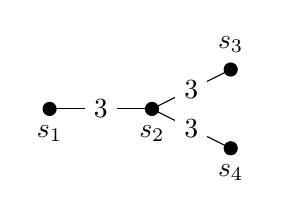
\begin{tikzpicture}
\node[draw,shape=circle,fill=black,scale=0.5](a)[label=below: {$s_1$}] at (-0.3,0) {};
\node[draw,shape=circle,fill=black,scale=0.5](b)[label=below: {$s_2$}] at (1,0) {};
\node[draw,shape=circle,fill=black,scale=0.5](c)[label=above: {$s_3$}] at (2,0.5) {};
\node[draw,shape=circle,fill=black,scale=0.5](d)[label=below: {$s_4$}] at (2,-0.5) {};

\draw (b)--(a) node [midway, fill=white] {$3$};
\draw (c)--(b) node [midway, fill=white] {$3$};
\draw (b)--(d) node [midway, fill=white] {$3$};
\end{tikzpicture}
\hspace{0.5in}
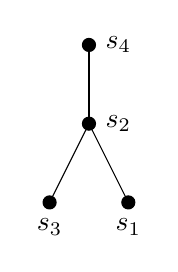
\begin{tikzpicture}
\node[draw,shape=circle,fill=black,scale=0.5](a)[label=right: {$s_2$}] at (0,0) {};
\node[draw,shape=circle,fill=black,scale=0.5](b)[label=below: {$s_1$}] at (0.5,-1) {};
\node[draw,shape=circle,fill=black,scale=0.5](c)[label=below: {$s_3$}] at (-0.5,-1) {};
\node[draw,shape=circle,fill=black,scale=0.5](d)[label=right: {$s_4$}] at (0,1) {};

\draw (b)--(a);
\draw (c)--(a);
\draw (a)--(d);
\end{tikzpicture}
\caption{The Coxeter diagram (left) for the Weyl group of type $D_4$. The fully commutative element $w=s_4s_2s_3s_1$ has heap poset $H_w$ shown on the right with $S$-labels; this example is an equality case $b([\id,w]_L)=\bi(H_w)=\frac{1}{3}$.}
\label{fig:type-D-equality}
\end{figure}


\begin{figure}[ht!]
\centering
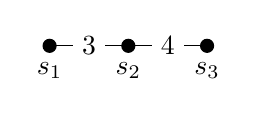
\begin{tikzpicture}
\node[draw,shape=circle,fill=black,scale=0.5](a)[label=below: {$s_1$}] at (0,0) {};
\node[draw,shape=circle,fill=black,scale=0.5](b)[label=below: {$s_2$}] at (1,0) {};
\node[draw,shape=circle,fill=black,scale=0.5](c)[label=below: {$s_3$}] at (2,0) {};

\draw (b)--(a) node [midway, fill=white] {$3$};
\draw (c)--(b) node [midway, fill=white] {$4$};
\end{tikzpicture}
\hspace{0.5in}
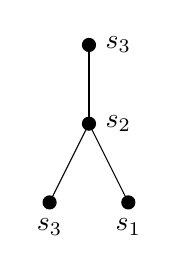
\begin{tikzpicture}
\node[draw,shape=circle,fill=black,scale=0.5](a)[label=right: {$s_2$}] at (0,0) {};
\node[draw,shape=circle,fill=black,scale=0.5](b)[label=below: {$s_1$}] at (0.5,-1) {};
\node[draw,shape=circle,fill=black,scale=0.5](c)[label=below: {$s_3$}] at (-0.5,-1) {};
\node[draw,shape=circle,fill=black,scale=0.5](d)[label=right: {$s_3$}] at (0,1) {};

\draw (b)--(a);
\draw (c)--(a);
\draw (a)--(d);
\end{tikzpicture}
\caption{The Coxeter diagram (left) for the Weyl group of type $B_3$. The fully commutative element $w=s_3s_2s_3s_1$ has heap poset $H_w$ shown on the right with $S$-labels; this example is an equality case $b([\id,w]_L)=\bi(H_w)=\frac{1}{3}$.}
\label{fig:type-B-equality}
\end{figure}


\begin{figure}[ht!]
\centering
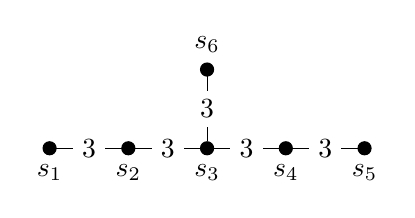
\begin{tikzpicture}
\node[draw,shape=circle,fill=black,scale=0.5](a)[label=below: {$s_1$}] at (0,0) {};
\node[draw,shape=circle,fill=black,scale=0.5](b)[label=below: {$s_2$}] at (1,0) {};
\node[draw,shape=circle,fill=black,scale=0.5](c)[label=below: {$s_3$}] at (2,0) {};
\node[draw,shape=circle,fill=black,scale=0.5](d)[label=below: {$s_4$}] at (3,0) {};
\node[draw,shape=circle,fill=black,scale=0.5](e)[label=below: {$s_5$}] at (4,0) {};

\node[draw,shape=circle,fill=black,scale=0.5](f)[label=above: {$s_6$}] at (2,1) {};

\draw (b)--(a) node [midway, fill=white] {$3$};
\draw (b)--(c) node [midway, fill=white] {$3$};
\draw (c)--(d) node [midway, fill=white] {$3$};
\draw (d)--(e) node [midway, fill=white] {$3$};
\draw (c)--(f) node [midway, fill=white] {$3$};
\end{tikzpicture}
\hspace{0.5in}
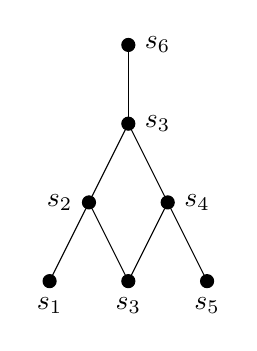
\begin{tikzpicture}
\node[draw,shape=circle,fill=black,scale=0.5](a)[label=below: {$s_1$}] at (-1,0) {};
\node[draw,shape=circle,fill=black,scale=0.5](b)[label=below: {$s_3$}] at (0,0) {};
\node[draw,shape=circle,fill=black,scale=0.5](c)[label=below: {$s_5$}] at (1,0) {};

\node[draw,shape=circle,fill=black,scale=0.5](d)[label=left: {$s_2$}] at (-0.5,1) {};
\node[draw,shape=circle,fill=black,scale=0.5](e)[label=right: {$s_4$}] at (0.5,1) {};

\node[draw,shape=circle,fill=black,scale=0.5](f)[label=right: {$s_3$}] at (0,2) {};

\node[draw,shape=circle,fill=black,scale=0.5](g)[label=right: {$s_6$}] at (0,3) {};

\draw (a)--(d)--(b)--(e)--(c);
\draw (d)--(f)--(e);
\draw (f)--(g);
\end{tikzpicture}
\caption{The Coxeter diagram (left) for the Weyl group of type $E_6$. The fully commutative element $w=s_6s_3s_2s_4s_1s_3s_5$ has heap poset $H_w$ shown on the right with $S$-labels; this example is an equality case $b([\id,w]_L)=\bi(H_w)=\frac{1}{3}$.}
\label{fig:type-E-equality}
\end{figure}

\begin{quest}
Let $w$ be a fully commutative element in a finite Weyl group with
\[
b([\id,w]_L)=\bi(H_w)=\frac{1}{3}.
\]
Is $H_w$ isomorphic to a disjoint union of the heap posets appearing in Figures \ref{fig:type-A-equality}, \ref{fig:type-D-equality}, \ref{fig:type-B-equality}, and \ref{fig:type-E-equality}?
\end{quest}

\section*{Chamber model}
For $D \subseteq A \subseteq T$ we write $W_D^A$ for the set of elements in $W$ whose right inversion set lies between $D$ and $A$:
\[
W_D^A=\{w \in W \: | \: D \subseteq T_R(w) \subseteq A\}.
\]

\begin{theorem}[Tits \cite{Tits}]
\label{thm:tits-convexity}
A set $C \subseteq W$ is left convex if and only if it is of the form $W_D^A$ for some $D \subseteq A \subseteq T$.
\end{theorem}

For $w\in W(\Phi)$, its \emph{inversion set} is $I_{\Phi}(w)=\{\alpha\in\Phi^+\:|\: w\alpha\in\Phi^-\}$; this is in bijection with $T_R(w)$ via the map $\alpha \leftrightarrow s_{\alpha}$ and we therefore sometimes write $C_{\alpha}$ for $C_{s_{\alpha}}$ and $\delta_C(\alpha)$ for $\delta_C(s_{\alpha})$.  For $A \subseteq \Phi^+$ we also write $W^A$ for the convex set $W^{\{s_a \: | \: a \in A\}}$ defined in Section~\ref{sec:background-cox-groups}. The \emph{Coxeter arrangement} is the central hyperplane arrangement in $E$ consisting of the hyperplanes
\[
H_{\alpha}\coloneqq\{x\in E\:|\:\langle x,\alpha\rangle=0\}
\]
for each $\alpha\in\Phi^+$. Regions of the Coxeter arrangement are called \emph{Weyl chambers} and are in bijection with the Weyl group $W$ in the following manner: for $w\in W$, the corresponding open Weyl chamber is
\[
R_w\coloneqq\{x\in E\:|\: \langle x,\alpha\rangle>0\text{ for }\alpha\in\Phi^+\setminus I_{\Phi}(w),\langle x,\alpha\rangle<0\text{ for }\alpha\in I_{\Phi}(w)\}.
\]
In particular, the \emph{fundamental Weyl chamber} $R_{\id}$ is $\{x\in E\:|\:\langle x,\alpha\rangle>0,\alpha\in\Phi^+\}$. It is now clear that the left Cayley graph $\cay_L(W)$ on $W$ is the same as the graph on the Weyl chambers where $R_w$ is connected to $R_u$ if and only if they are separated by a single hyperplane $H_{\alpha}$. As a result, $C\subseteq W$ is left convex if and only if $\bigcup_{w\in C}\overline{R_w}$ is a convex polyhedron. This geometric perspective will be used in Section~\ref{sec:bounds-Weyl}.

\section*{Uniform lower bound and the geometric input}
\begin{theorem}\label{thm:uniform-bound}
There exists an absolute constant $\epsilon>0$ such that for any non-singleton convex set $C$ in any finite Weyl group we have
\[
b(C)>\epsilon.
\]
\end{theorem}

\begin{cor}\label{cor:bm}
Let $Q\subseteq\R^n$ be a full-dimensional compact convex body with centroid $c_Q$. Let $m\geq1$ and $v\in\R^n$ be such that $\langle v,c_Q\rangle\geq\frac{-m}{n+1}$. Suppose that $\min_{x\in Q}\langle v,x\rangle\leq-1$ and $\max_{y\in Q}\langle v,y\rangle\geq1$. Then
$\frac{\Vol(Q_v^+)}{\Vol(Q)}\geq\frac{1}{2e^m}.$
\end{cor}

\begin{table}[ht!]
\centering
\begin{tabular}{|c|c|c|c|c||c|c|}
\hline
Type & $m_0$ & $m_1$ & $\height(\Phi)$ & $m$ & $mm_1$ & $b(C)\geq$\\\hline
$A_r$ & 1 & 1 & $r$ & 1 & 1 & $1/2e$  \\\hline
$B_r$ & 1 & 2 & $2r-1$ & 1 & 2 & $1/2e^2,1/2e$ \\\hline
$C_r$ & 1 & 2 & $2r-1$ & 1 & 2 & $1/2e^2,1/2e$ \\\hline
$D_r$ & 1 & 2 & $2r-3$ & 2 & 4 & $1/2e^4$\\\hline
$E_6$ & 1 & 3 & 11 & 8/3 & 8 & $1/2e^8$\\\hline
$E_7$ & 1 & 4 & 17 & 3 & 12 & $1/2e^{12}$\\\hline
$E_8$ & 2 & 6 & 29 & 7/4 & 21/2 & $1/2e^{10.5}$\\\hline
$F_4$ & 2 & 4 & 11 & 7/8 & 7/2 & $1/2e^{3.5}$ \\\hline
$G_2$ & 2 & 3 & 5 & 1/2 & 5/2 & $1/2e^{2.5}, 1/3$ \\\hline
\end{tabular}
\caption{The parameters and bounds appearing in Theorem~\ref{thm:uniform-bound-specific} for each irreducible type.  The second listed lower bounds for types $B_r$ and $C_r$ follow from Theorem~\ref{thm:typeB-better-bound}, while the bound of $1/3$ for type $G_2$ is immediate for any rank-two Coxeter group.}
\label{tab:centroid-data}
\end{table}
\end{document}
